% STILL TO DO


\documentclass{report}
\usepackage{filecontents}

\usepackage[utf8]{inputenc}
\usepackage[T1]{fontenc}
\usepackage[francais]{babel}
\usepackage{listings}
\usepackage[a4paper]{geometry}
\usepackage{graphicx}
\usepackage[export]{adjustbox}
\usepackage{titlesec}
\usepackage{color}
\usepackage[toc, page]{appendix}
\usepackage{url}

\definecolor{xcodekw}{rgb}{0.75, 0.22, 0.60}
\definecolor{xcodestr}{rgb}{0.89, 0.27, 0.30}
\definecolor{xcodecmt}{rgb}{0.31, 0.73, 0.35}

\titleformat{\chapter}[display]
  {\centering\normalfont\huge\bfseries}
  {\chaptertitlename\ \thechapter}
  {20pt}
  {\Huge}

\geometry{hscale=0.75,vscale=0.85,centering}

\renewcommand{\thesection}{\arabic{section}}
\renewcommand\appendixtocname{Annexes}
\renewcommand\appendixname{Annexes}
\renewcommand\appendixpagename{Annexes}

\title{Architecture des Bases de Données\\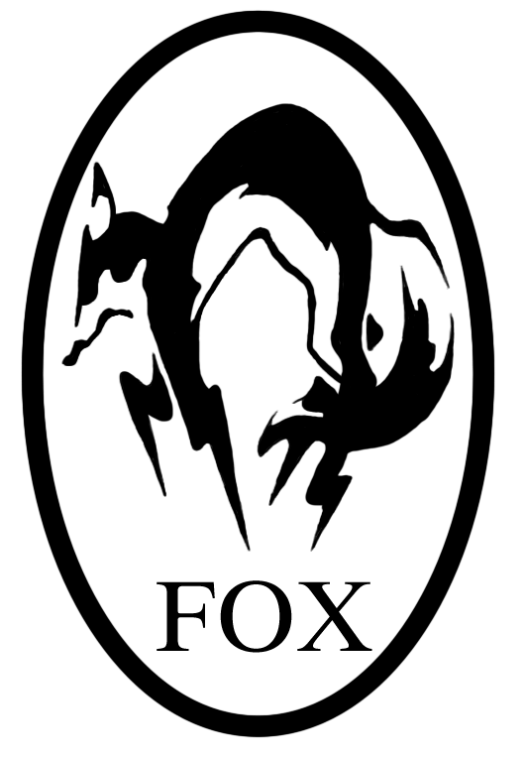
\includegraphics[scale=0.3]{foxhound.png}}
\author{Samuel "Big Boss" \bsc{Monroe}}

\date{\today}

\begin{document}

\maketitle

\newpage
\thispagestyle{empty}
\mbox{}

\tableofcontents

\chapter{Avant-Propos}

	Voici la synthèse pure ultime qui va fournir une vision pure et complète du cours de Mr. Faulkner afin que tu ne te fasses pas déchirer la raie à l'examen, sauf si tu n'as rien fait pour les projets mon asti.\\

\chapter{Démarche d'Analyse et de Modélisation d'un Système d'Information}

	L'ensemble du cours d'Architecture des Bases de données avait pour but de faire progresser l'étudiant dans cette démarche d'analyse et de modélisation.\\
	Cette synthèse va donc suivre cette démarche, en revenant sur la découpe et le cheminement du processus, nous verrons ensuite individuellement chacune des étapes qui a été accomplie, et nous terminerons par une analyse supplémentaire de ces étapes afin de lier celles-ci entre elles et parfaire la vision globale de la démarche.\\

	\section{Découpe des étapes}

		Pour l'instant, nous allons décomposer ce travail en trois grosses étapes, qui seront également les trois chapitres qui vont suivre : \\

		\begin{enumerate}
			\item \textbf{Database} : Cette étape reprend principalement la réalisation du \textbf{schéma entité-association}, du \textbf{schéma relationnel} et du \textbf{Data-Definition Language}.
			\item \textbf{Application} : Dans cette étape, le but à atteindre est l'obtention d'une base prête l'emploi pour implémentation du produit, mais aussi d'autres que nous détaillerons plus tard. Les étapes de la démarche sont ici la réalisation de \textbf{Use-Case Models}, de \textbf{Scénarii} qui vont appuyer ces use-cases, ensuite viennent les \textbf{diagrammes d'activités} qui vont terminer la base nécéssaire à la création d'un \textbf{diagramme de classe}, enfin le \textbf{diagramme de séquence} viendra corriger et compléter ce diagramme de classe.\\
			\item \textbf{Design - Visualisation} : A partir du diagramme de classe, ce sont les \textbf{objets} qui doivent être créés. Il y a enfin la réalisation de \textbf{Mockups} afin de terminer cette démarche et préparer l'implémentation réelle.\\
		\end{enumerate}


\chapter{Database}

	Cette étape du travail est effectuée à partir d'une situation réelle décrite, et pour laquelle le but final est de fournir un \textbf{Système d'Information} qui répondra aux besoins identifiés par la situation.\\

	Le but de la partie Database est de fournir une structure de données exploitable pour la suite de la démarche d'Analyse et de Modélisation.\\

	On peut découper cette démarche Database de la sorte : \\

	\begin{enumerate}
		\item A partir de l'\textbf{énoncé}, on effectue une \textbf{analyse conceptuelle} afin de créér un \textbf{schéma conceptuel}.\\
		\item A partir de ce même \textbf{schéma cocneptuel}, on produit un \textbf{schéma de base de données}, qui fournira ensuite le SQL.\\
	\end{enumerate}

	\section{Schéma Entité-Association}

		En tout premier lieu, il convient d'Analyser le \textbf{Case-Study} afin d'en repérer toutes les entités intervenantes et les associations entre celles-ci.\\

		Ce modèle fournit un monde formé d'entités, ayant des propriétés (\textbf{attributs}) et en association les unes avec les autres. Ce \textbf{monde} est notre cas décrit, appelé aussi \textbf{le domaine d'application}.\\

		\subsection{Entités}

			Les entités représentent les objets du domaine d'application, qui possèdent eux-mêmes des propriétés ou attributs qui le définissent.\\
			Ces entités sont représentées de la manière suivante, un cadre portant le nom de l'entité et comportant ses attributs : \\

			\includegraphics[scale=0.6]{entity.png}\\

		\subsection{Associations}

			Ces entités sont liées entre elles par des associations.\\

			Ces associations portent un nom représentant le type, de préférence un verbe bien spécifique (pas être ou avoir), et les entités peuvent posséder un nom de \textbf{rôle} implicite ou explicite sur cette association : \\

			\includegraphics[scale=0.6]{role.png}\\

			Ces associations ont également une \textbf{cardinalité} qui complète leur type, elle définit sur quelle base numérique va s'effectuer l'association, c'est-à-dire combien d'entités A sont en association avec l'entité B.\\
			Selon les standards, cette cardinalité se lit en commencant par l'élément le plus éloigné.\\
			On retrouve plusieurs types d'associations : \\

			\subsubsection{Un-à-plusieurs}

				Aussi appelée \textbf{1:N}, elle se lit ici : "Un département emploie N employés"\\
				Ou bien de point de vue d'un employé : "N Employés sont occupés par 1 (seul) département"\\

				\includegraphics[scale=0.6]{oneton.png}\\

			\subsubsection{Un-à-Un}

				Ou \textbf{1:1}, on lira ici : "Un département dirige un employé"\\

				\includegraphics[scale=0.6]{onetoone.png}\\


			\subsubsection{N à N}

				Ou \textbf{N:N}, on lira ici : "Plusieurs usines fabriquent plusieurs produits."\\

				\includegraphics[scale=0.6]{nton.png}\\

			\subsubsection{Rôles obligatoires ou facultatifs sur la cardinalité}

				Une cardinalité plus détaillée peut informer du caractère facultatif d'un rôle tel qu'on peut le voir ici : \\

				\includegraphics[scale=0.6]{facultatif.png}\\

			\subsubsection{Associations cycliques}

				Dans cette association, les deux rôles sont joués par le même type d'entité. A ne pas appeler \textbf{récursif} : \\

				\includegraphics[scale=0.6]{recursif.png}

		\subsection{Identifiants}

			On repére les entités d'une population par un ou plusieurs attributs qui seront son ou ses identifiant, et notés de la façon suivante :\\

			\includegraphics[scale=0.]{identifiants.png}\\

			Pour les relations 1 à 1, l'identifiant d'une entité peut-être implicite de la manière suivante : \\

			\includegraphics[scale=0.6]{implicite.png}\\

			Un identifiant peut aussi être hybride de part une relation multiple : \\

			\includegraphics[scale=0.6]{hybride.png}\\

		\subsection{Cas concret}

			Voici un exemple concret d'un petit schéma E-A d'une gestion de bibliothèque : \\

			\includegraphics[scale=0.6]{bibli.png}\\


	\section{Schéma Relationnel}

		Cette étape du travail va essentiellement consister à reprendre le schéma \textbf{Entité-Association} et à transformer nos associations pour produire un schéma \textbf{relationnel}.\\
		Comme nous allons le voir juste après, nos associations vont se transformer en identifiants supplémentaires qui vont exprimer ces associations d'une manière exploitable pour produire le DDL(SQL).\\

		\subsection{Transformation d'attributs composés}

			La première étape consiste en la transformation des attributs composés, telle l'adresse contenue dans une autre entité.\\

			Ceci peut-être accompli par : \\

			\begin{itemize}
				\item Désagration, on remplace l'attribut par ses composants dans la même entité
				\item Transformation en types d'entités instanciés, dans laquelle la nouvelle entité adresse est directement liée à l'autre entité en possédent le même identifiant. Ceci est le cas pour les relations 1:1
				\item Transformation en types d'entités par valeurs, la nouvelle entité est "indépendante", possède son propre identifiant, c'est dans l'autre entité que l'on va placer un champ destiné à identifier à quelle(s) addresse(s) elle est reliée.\\
			\end{itemize}

			Voici un exemple pour des attributs composés obligatoires : \\

				\includegraphics[scale=0.5]{attobli.png}\\

			Et pour des facultatifs : \\

				\includegraphics[scale=0.5]{attfacu.png}\\	

		\subsection{Transformation d'associations}

			Il y a lieu à présent de transformer les associations en identifiants supplémentaires.\\

			Basiquement cette transformation est la suivante : \\

			\includegraphics[scale=0.6]{trans.png}\\

			Le caractère facultatif d'une relation 0:1 est exprimé par un \textbf{ref} dans l'id, tandis que l'obligation s'exprime par \textbf{eq}.\\

			Certaines associations peuvent mener à la création de nouvelles tables, typiquement pour les relations 0:N ou 1:N, mais pas seulement : \\

			\includegraphics[scale=0.6]{newentity.png}\\

			Pour les relations cycliques, l'association peut également se transformer en nouvelle table pour une association 0:N, ou en reférences pour une relation 0:1 : \\

			\includegraphics[scale=0.6]{cyclique.png}\\

		\section{DDL}

			Maintenant que l'on possède le schéma relationnel, il s'agira uniquement de traduire ces boxes en tables via le langage SQL, typiquement de la manière suivante : \\

			\includegraphics[scale=0.7]{ddl.png}

\chapter{Application}

	Ce chapitre va s'attarder sur la partie liée à l'application en elle-même, maintenant que nous possèdons la partie base de données.\\

	Nous allons d'abord voir le \textbf{Use Case Model}, ensuite les \textbf{Scénarios} duquel nous tirerons les \textbf{Activity Diagrams}. De là nous tirerons un \textbf{Diagramme de Classe} qui sera étoffé par la réalisation finale d'un \textbf{Diagramme d'Interaction}.\\

	\section{Use Case Model}

		Le Use-Case model est un modèle décrivant le comportement de quelques entités telles que le système ou sous-systèmes, son comportement est la façon dont il agit et réagit.\\
		C'est aussi un modèle qui décrit les interactions du système avec son environnement.\\

		Ce Use-Case va permettre d'obtenir une communication facilitée entre l'expert et l'utilisateur, de permettre d'identifier les entités intervenantes et de pouvoir vérifier la validité du tout.\\

		\subsection{Concepts basique du Use-Case Diagram : Acteur}

			L'acteur représente un utilisateur agissant avec le système selon certains rôles, il peut être un humain, machine ou un autre système.\\
			Il peut échanger de l'information avec le système, être seulement donateur d'information, ou receveur passif d'information.\\
			Les acteurs sont externes.\\

		\subsection{USer-Case Diagram : Use-Case}

			Le Use-Case en liu-même décrit une séquence d'actions qu'un système effectue afin d'obtenir un résultat observable par rapport à un acteur.\\
			Cette séquence d'action peut être décrite informellement dans du texte ou dans la spécification du comportement représentée par un lien vers un diagramme d'interaction.\\

			Ces Use-Case sont représentés dans le diagramme par une bulle ovale portant le nom associé.\\

			Les \textbf{Scénarios} sont utilisant pour référencer le déroulement des choses que peuvent prendre différentes instances possibles d'un même Use-Case.\\

		\subsection{Relation entre l'acteur et le use-case}

			Un Use-Case est initié par un acteur qui souhaite invoquer une fonctionnalité du système, l'acteur est connecté aux use-cases avec lesquels il interagit par une relation de communication.\\

			\includegraphics[scale=0.6]{ucrelation.png}\\

		\subsection{Use-Case description}

			Généralement, un indication sur les scénarios couverts et les champs accédés sera ajoutée, le use-case description se présente en colonnes entre lesquelles les acteurs vont établir des actions.\\

			\includegraphics[scale=0.6]{ucdescription.png}

		\subsection{Autres types de relations}

			On trouve : \\

			\begin{enumerate}
				\item Généralisation entre use-cases (inherits)
				\item Généralisation entre acteurs (inherits)
				\item Relation d'inclusion (uses)
				\item Relation d'extension (extends)
			\end{enumerate}

	\section{Diagramme d'activité}

		Le diagramme d'activité est un moyen de décrire le fonctionnement d'un business, des uses-cases en eux-mêmes et entre eux.\\

		Ce diagramme consiste en activités, état et transisitions entre ces activités et ces états.\\

		\begin{itemize}
			\item L'activité est une spécification du comportement exprimée en flux d'actions
			\item L'état est un point où un évènement doit avoir lieu pour que l'activité continue
			\item La transition est un mouvement entre activités et ou états, elle est supposée représenter des actions qui surviennent rapidement et qui sont non-interruptibles.\\
		\end{itemize}

		On trouve des diagrammes d'activités qui décrivent un use-case, d'autres qui décrivent les opérations.\\

		\subsection{Activités}

			Les activité sont une unité de travail, ce travail peut être mentionné dans l'activité afin de bien signifier l'action entreprise.\\

			\includegraphics[scale=0.8]{activity.png}\\

			Les actions peuvent être déclanchées par entrée lorsque l'activité commence, simplement lors du temps de vie de l'activité, lors d'un évènement, ou lors de la fin d'un évènement.\\

		\subsection{Etats}

			Ils signifient une étape d'attente, on trouve également deux états spéciaux de fin (bulle noire entourée) et de début (bulle noire) de diagramme.\\

		\subsection{Transitions}

			Les transitions sont effectuées à la fin d'une activité, celle-ci peut être non déclanchée et survient naturellement, ou doit être déclanchée pour sortir d'un état d'attente par exemple.\\

			On peut également trouver de multiples transition, aussi déclanchée ou non.\\

			Une transition peut être \textbf{forkée}. Cela signifie que deux chemins parallèles vont être suivis en même temps, ces chemins peuvent se rejoindre sur un \textbf{join}.\\

		\subsection{Points de décisions}

			Point du diagramme ou un choix est effectuée sur base de conditions.\\

		\subsection{Exemple de diagramme d'activité complet}

			Dans ce diagramme, on observe aussi l'apparition d'objets pour identifier lesquels sont effectés par un flux.\\

			\includegraphics[scale=0.6]{adiagram.png}

	\section{Diagramme de classe}

		Le diagramme de classe décrit une structure statique des classes qui agissent avec le système.\\
		Cette structure statique inclus les classes, leurs attributs et opérations ainsi que les relations entre elles.\\

		Les classes qui sont montrées sur le diagramme dépendent de la phase de développement et du niveau de détail souhaité.\\

		Les diagrammes de classe sont utilisés pour documenter les classes qui constituent le système ou le sous-système, pour décrire les associations, généralisations et agrégations entre ces classes.\\
		Pour montrer les attributs et opérations de chaque classe, pour montrer la structure d'une classe au long du cycle de vie du développement.\\
		Pour montrer les objets individuels dans une structure de classe ainsi que pour montrer les interfaces supportées par une classe donnée.\\

		Je passerai ici les éléments déjà vu en Java concernant les classes et objets et m'attarderai sur des concepts un peu plus importants.\\

		\subsection{Généralisation}

			Relation d'héritage représentée par un triangle, la classe parent est la classe généralisée, les enfants sont les classes spécialisées et héritent du parent.\\
			Les enfants peuvent redéfinir les méthodes afin de les utiliser selon la spécialisation.\\

		\subsection{Classification Dynamique}

			La classification refère aux relations entre un objet et les classes dont il est une instance.\\

			Certaines classification sont dites \textbf{mandatoires} ce qui signifie qu'une classe doit être une instance de telle classe, d'autres sont dites dynamique et peuvent cesser d'être une instance de telle classe pour devenir une autre.\\

		\subsection{Relation d'association}

			Une association est une relation structurée qui représente une relation binaire entre des objets, une association a un nom et doit être spécifiée de zéro, un ou deux rôles.\\

			Une cardinalité peut être ajoutée à l'association (pas même sans que E-A !), et une direction peut-être apposée au nom.\\

		\subsection{Agrégation}

			L'agrégation est une relation d'appartenance, ou un objet est un tout, et l'autre est une partie du premier.\\

			Cette relation est marquée d'un losange : \\

			\includegraphics[scale=0.5]{aggregation.png}\\

		\subsection{Composition}

			Cas spécial de l'aggrégation, une relation de composition implique une relation vie/mort entre les deux classes. Si une instance meurt, les instances liées à la composition doivent mourrir elles aussi.\\

			\includegraphics[scale=0.6]{composition.png}\\

		\subsection{Business Rules}

			Une Business Rule est utilisée pour décrire les propriété d'une application, par exemple le fait qu'un employé ne peut gagner plus que son manager.\\

			Elle peut être : \\

			\begin{itemize}
				\item Description d'un concept ayant un rapport avec l'application
				\item Une contrainte d'intégrité sur les données de l'application
				\item Une règle dérivée, où l'information peut être dérivée d'une autre information dans le diagramme de classe
			\end{itemize}


	\section{Diagramme d'interaction}

		En object-oriented les tâches du système sont effectuée par des objets interagissant ensemble.\\
		Les interactions entre ces objets sont modélisées par des diagrammes d'interaction.\\
		Une interaction entre deux objets A et B implique que A envoie un message qui requière une action que B peut effectueur.\\

		Il y a deux types de diagrammes d'interaction : \\

		\begin{itemize}
			\item Les diagrammes de séquences
			\item Les diagrammes de collaboration\\
		\end{itemize}

		Le diagramme de classe modélise la structure statique du système tandis que le diagramme d'interaction modélise la partie dynamique.\\

		\subsection{Diagrammes de Séquences}

			Les diagrammes de séquences décrivent en détails comment les acteurs utilisent les use-cases.\\
			Les interactions consistent en un ou plusieurs messages échangés entre des objets externes et faisant partie du système.\\
			Les interactions peuvent être synchrones ou asynchrones.\\

			Voici un exemple complet de diagramme de séquence : \\

			\includegraphics[scale=0.6]{seq.png}\\

		\subsection{Contrôle de flux}

			Des flêches pointillées optionnelles peuvent être ajoutées pour représenter les retours après appels de méthodes.\\

		\subsection{Comment produire un diagramme de séquence}

			Pour un cas particulier, commencer par identifier les objets et acteurs impliqués.\\

			Elaborer pas à pas le diagramme de séquence.\\

			Retourner à la définition de la classe pour repérer les attributs ou méthodes qui manqueraient.\\

		\subsection{Relations avec les autres diagrammes}

			Le diagramme de séquence peut être utilisé pour vérifier les use-cases ou les classes.\\

		 	\begin{itemize}
		 		\item Chaque opération du diagramme de séquence doit exister dans le diagramme de classe
		 		\item Le nom des messages doit être un évènement ou une méthode de la classe qui recoit ce message\\
		 	\end{itemize}

\chapter{Schéma Récapitulatif}

	\includegraphics[scale=0.7]{schema.png}

\end{document}